
%!TEX root = Main.tex
\documentclass[a4paper,11pt,twoside]{article}  %{report} / article
% Alternative Options:
% Paper Size: a4paper / a5paper / b5paper / letterpaper / legalpaper / executivepaper
% Duplex: oneside / twoside
% Base Font Size: 10pt / 11pt / 12pt
 
%% Language
\usepackage[english]{babel} %francais, polish, spanish, 
\usepackage[T1]{fontenc}	   %character encoding of the .pdf files (?)
\usepackage[utf8]{inputenc} %character encoding of the .tex files

\usepackage{lipsum}

%\usepackage{lmodern} %Type1-font for non-english texts and characters

%\usepackage{mathpazo}
\usepackage{setspace}

\usepackage{palatino}
\usepackage{helvet}                 %load a helvetica font

\usepackage[EULERGREEK]{sansmath}	%sans serif font for math mode

\usepackage{marvosym} %symbols

\usepackage{microtype}  %character spacing usw. (load after font)


\usepackage{fixltx2e}   % fixes some small errors in LaTeX2e

%% Page Format
\usepackage[a4paper]{geometry}
%\geometry{left=20mm, right=20mm, bindingoffset=10mm}
\geometry{left=20mm, right=20mm}
\geometry{tmargin=33mm,bmargin=30mm}

%\usepackage{setspace}	%Linespacing
%\singlespacing (default) // \onehalfspacing // \doublespacing // \linespread{2}

%% DEFINE ACRONYMS
%\usepackage[printonlyused, nohyperlinks,nolist]{acronym} %the acronym package

%\usepackage{makeidx}
%\makeindex


%% Packages for Graphics & Figures
\usepackage{graphicx}		%For loading graphic files

%\usepackage{epstopdf}		%To automatically convert .eps to .pdf graphics
\usepackage{xcolor}			%color handling

% tikz -> Generate vector graphics from within LaTeX
\usepackage{tikz}
%\usepackage{tikz-3dplot}
%\usetikzlibrary{arrows,matrix,positioning,fit,petri,calc}
%\usetikzlibrary{chains}
%\usetikzlibrary{decorations}

% pgfplots -> make plots with tikz
\usepackage{pgfplots}
%\pgfplotsset{compat=newest}
%\usetikzlibrary{pgfplots.statistics}
%\usetikzlibrary{plotmarks}

% set sans serif font for pgf plots
%\pgfplotsset{
%  tick label style = {font=\sansmath\sffamily},
%  every axis label = {font=\sansmath\sffamily},
%  legend style = {font=\sansmath\sffamily},
%  label style = {font=\sansmath\sffamily}
%}

%\pgfplotsset{
%tick label style={font=\scriptsize},
%label style={font=\small},
%legend style={font=\tiny}
%}

%\pgfkeys{
%   /pgf/number format/.cd, 
%      set decimal separator={.},
%      set thousands separator={}
%}


%\pgfplotsset{colormap={redblue}{color(0cm)=(green) color(0.1cm)=(blue) color(2.5cm)=(white) color(4.9cm)=(red) color(5cm)=(yellow)}}



% redefine how figure & table captions look
\usepackage[hypcap]{caption}
\captionsetup{font=small,labelfont=bf,textfont=it}

% (a) (b) subcaptions for figures
% \usepackage{subcaption}

% figures with the caption to one side
\usepackage{sidecap}

\usepackage{float} %the H command

% "LaTeX => PDF" allows: .jpg  .png  .pdf  .mps
% "LaTeX => DVI", "LaTeX => PS" und "LaTeX => PS => PDF": allow the following formats: .eps  .ps  .bmp  .pict  .pntg


%% Biblography
\usepackage{natbib}


%backend=bibtex
%backend=biber
%\usepackage[backend=bibtex,natbib=true,style=apa,hyperref=true,backref=true,            block=none]{biblatex}
%\addbibresource{Bibliography.bib}% 



%% TABLES
\usepackage{tabularx}		% for fancy tables
\usepackage{multirow}		%for multiple rows in a table
\usepackage{multicol} 		%multible columns
\usepackage{booktabs}		%for top/ midrule usw.
\usepackage{array}			%more possibilities for tables


%% SCIENCE
\usepackage{mathtools}			% loads amsmath
\usepackage{siunitx}				% SI units
% \usepackage[version=3]{mhchem}	% For chemical formulae

% Programming
% \usepackage{listings}	%Code environnements
% \usepackage[framed,numbered,autolinebreaks]{mcode} %for matlab looking code

% auto detect end of macro
\usepackage{xspace}

\usepackage{xifthen}


% Headers and Footers

%\usepackage{floatpag} %for \(this)floatpagestyle

%get the number of the 'part' in the header
%\newcommand*\parttitle{}
%\let\origpart\part
%\renewcommand*{\part}[2][]{%
%   \ifx\\#1\\% optional argument not present?
%      \origpart{#2}\thispagestyle{empty}%
%      \renewcommand*\parttitle{\thepart~#2}%
%   \else
%      \origpart[#1]{#2}\thispagestyle{empty}%
%      \renewcommand*\parttitle{\thepart~#1}%
%   \fi
%}

\usepackage{fancyhdr}
%\usepackage{emptypage}
%\renewcommand{\sectionmark}[1]{\markboth{#1}{}}

\fancyhf{}
%\renewcommand{\part}{\part\thispagestyle{empty}}
\pagestyle{fancy}

%\renewcommand{\chaptermark}[1]{\uppercase{\markboth{#1}{}}}
\renewcommand{\sectionmark}[1]{\uppercase{\markboth{#1}{}}}

%\renewcommand{\chaptermark}[1]{ \markboth{#1}{} }
%\renewcommand{\sectionmark}[1]{ \markright{#1}{} }

\addtolength{\headheight}{2pt}
%\fancyhead[LE,RO]{\thepage}
%\fancyhead[LO,RE]{{\parttitle}}
%\fancyhead[LO,RE]{\thechapter~{\leftmark}}
\fancyhead[C]{\textsc{\leftmark}}
%\fancyhead[CO]{\rightmark}
\fancyfoot[C]{\thepage}
%\fancyfoot[LO,RE]{\monthword{\the\month}~\the\year}
%\renewcommand{\headrulewidth}{0.5pt}
%\renewcommand{\headrulewidth}{0pt}

%\renewcommand{\footrulewidth}{0.5pt}



% REDEFINE STYLE OF EMPTY PAGES (CLEARDOUBLEPAGE)
% only page number

% \leardoublepage -> style: plain

\makeatletter
\def\cleardoublepage{\clearpage\if@twoside \ifodd\c@page\else
\hbox{}
%\vspace*{\fill}
%\begin{center}
%This page intentionally contains only this sentence.
%\end{center}
%\vspace{\fill}
\thispagestyle{plain}
\newpage
\if@twocolumn\hbox{}\newpage\fi\fi\fi}
\makeatother


%footnotes look crappy with \raggedbottom
\usepackage[bottom]{footmisc}



%stops a the contents of a unfilled page being spread over the whole page but confines it to the upper part
\raggedbottom


%!TEX root = Main.tex

%define graphics path:
\graphicspath{{./figures/}}



\setlength{\unitlength}{\textwidth}
%% DEFINE NEW SI UNITS


\DeclareSIUnit{\Wm}{\watt \per \meter \squared}


%Brakets (or square Brackets) 
\DeclareSIUnit{\rB}{\ensuremath{]}}
\DeclareSIUnit{\lB}{\ensuremath{[}}

%Parantheses
\DeclareSIUnit{\rP}{\ensuremath{)}}
\DeclareSIUnit{\lP}{\ensuremath{(}}

\DeclareSIUnit{\div}{\ensuremath{/}}

\sisetup{separate-uncertainty=true}

\sisetup{detect-all=true}
\sisetup{retain-explicit-plus=true}

% good looking units in captions
\newcommand{\capunit}[1]{\si[detect-all=false]{\lB#1\rB}}


% example commands
% \newcommand{\p}[1]{\ensuremath{\text{p}_{#1}}} %percentile
% \newcommand{\sunel}{\ensuremath{\theta_e}\xspace}
% \newcommand{\KZ}{K\&Z\xspace}


% dot for f(.)
\newcommand*{\edot}{\makebox[1ex]{\textbf{$\cdot$}}}%

\newcommand{\hl}[2]{\ensuremath{\text{#1}_{\text{#2}}}}

\newcommand{\gridRes}[2]{\SI{#1}{\degree} $\times$ \SI{#2}{\degree}}

%% COMMANDS


% \fig{(b)}{fig_name}
\newcommand{\fig}[2][]{%
Figure~\ref{fig:#2}\ifthenelse{\isempty{#1}}{}{(#1)}%
}

%\newcommand{\fig}[1]{Figure~\ref{fig:#1}}
%\eqref{} defined by amsmath
\newcommand{\tab}[1]{Table~\ref{tab:#1}}
\newcommand{\sect}[1]{Section~\ref{#1}}
\newcommand{\chap}[1]{Chapter~\ref{#1}}


%% TABLES
\newcolumntype{C}[1]{>{\centering\arraybackslash}p{#1}}
\newcolumntype{L}[1]{>{\raggedright\arraybackslash}p{#1}}

% FIGURES
\newcommand{\singlefig}[2]{%
\begin{figure}[h!tbc]
        \centering
        \includegraphics[width=\textwidth]{#1}
			\caption{#2 \label{fig:#1}}
\end{figure}
}




\newcommand{\doublefig}[4]{%
\begin{figure}[h!tbc]
        \centering
              \begin{minipage}[t]{0.48\textwidth}
                \centering
                \includegraphics[width=\textwidth]{#1}
				\captionof{figure}{#2 \label{fig:#1}}
        \end{minipage}%
		\hfill
\begin{minipage}[t]{0.48\textwidth}
                \centering
                \includegraphics[width=\textwidth]{#3}
				\captionof{figure}{#4 \label{fig:#3}}
        \end{minipage}%
\end{figure}
}


\numberwithin{figure}{subsection}
\numberwithin{table}{section}

%\renewcommand{\thefigure}{\thesection.\arabic{figure}}

% the automatic references (ought to be the last package)
\usepackage[plainpages=false,pdfpagelabels]{hyperref}
\begin{document}
%\input{DefinitionAcronyms}

%!TEX root = Main.tex
\thispagestyle{empty}

%\begin{table}[h]\huge
%   \centering
%   \begin{tabular}{c}
%	Master Thesis Proposal\\ 
%     \toprule
% 	\textbf{Soil Carbon -- Climate Feedback} \\
%  \end{tabular}
% \end{table}

\begin{center}
	\begin{LARGE}
\textsc{Article}\\ % -- Mathias Hauser\\
\noindent\rule[1ex]{\textwidth}{0.8pt}  %{1.1pt} 
\newline
%\vspace*{1ex}
\textbf{{
The Title
}}  \\[1ex]
\noindent\rule[1ex]{\textwidth}{0.8pt} %{1.1pt}
%Mathias Hauser\\
	\end{LARGE}
%mathause@ethz.ch\\
\end{center}

%\begin{figure}[h!tbc]
	%\centering
%\input{./tikz/tikzPools}
%\end{figure}

\vfill
\begin{center}
	\large
\textbf{Name}\\(\Letter{}) xx@xx.ch \\[0.5cm]
\textbf{Supervision:}\\
Prof.\ Dr.\ Supervisior\\
\end{center}



\begin{center}
\large
Land-Climate Interactions Group \\ 
Institute for Atmospheric and Climate Science,  IAC\\
Eidgenössische Technische Hochschule Zürich, ETHZ\\[10pt]
%\\ %\noindent \newline
Zürich, Switzerland -- January 2015 \\%[20pt]
\end{center}

\vspace{20pt}


\noindent\begin{tabularx}{\textwidth}{lllX}
\vspace{.4in}
Research Plan accepted: &&&\\
Main Supervisor: & \makebox[1.5in]{\hrulefill} & \makebox[2in]{\hrulefill} &\\
\vspace{.4in}
& Date & Sonia Seneviratne&\\%[8ex]% adds space between the two sets of signatures
Doctoral Student: & \makebox[1.5in]{\hrulefill} & \makebox[2in]{\hrulefill}&\\
& Date & Mathias Hauser&\\
\end{tabularx}




%\begin{minipage}[t]{0.48\textwidth}
%\large
%\centering
%\textbf{Mathias Hauser}\\
%mathause@ethz.ch \\
%\end{minipage}
%\begin{minipage}[t]{0.48\textwidth}
%\large
%\centering
%\textbf{Supervision:}\\
%Prof.\ Dr.\ Sonia I.\  Seneviratne\\
%Benoît Guillod\\
%Dr.\ Edouard Davin
%\end{minipage}












\vspace{10pt}

\normalsize

%\flushright{\sffamily\Huge{{IAC\textit{\textbf{ETH}}}}}
\begin{figure}[H]
\centering
\begin{tikzpicture}[inner sep = 0pt]
	\node[inner sep = 0pt] {
\includegraphics[width=5.00 cm]{./figures/eth_logo_black.eps}};
	\node[anchor=north east, xshift = \textwidth,inner sep = 0pt] (ETH) at (current bounding box.north west) {\sffamily\Huge{{IAC\textit{\textbf{ETH}}}}};
\end{tikzpicture}
\end{figure}


\newpage


\setcounter{page}{1}
\pagenumbering{roman} 
\pagestyle{plain}
%!TEX root = Main.tex
\begin{figure}[c]

\centering
\begin{minipage}[H]{\textwidth} %{0.85\textwidth}

%\hspace*{20pt}
\section*{Abstract} \label{sec:Summary}
%\textbf

\end{minipage}

\end{figure}
\cleardoublepage


\tableofcontents 
\cleardoublepage
\setcounter{page}{1}
\pagenumbering{arabic}
\pagestyle{fancy}

%!TEX root = Main.tex

\section{Introduction}


\lipsum[15] See table \tab{SoilParam}


% \citet{Lawrence2008}

\begin{table}[h!tb]
\caption{Soil parameters as used in CLM for two typical soil types and a pure organic soil. \label{tab:SoilParam}}
{
\centering
\begin{tabular}{l c c c c c c c c}
\toprule
Soil type & $\lambda_{\text{s}}$ & $\lambda_{\text{sat}}$ & $\lambda_{\text{dry}}$ & $c_{\text{s}}$ & $\Theta_{\text{sat}}$ & $k_{\text{sat}}$ & $\Psi_{\text{sat}}$ & $b$ \\
& \multicolumn{3}{c}{\capunit{\watt}} &\capunit{\giga\joule\per\meter\cubed\per\kelvin }&\capunit{-}&\capunit{\milli\meter\per\second}&\capunit{\milli\meter}&\capunit{-} \\
\midrule
Sand$^*$  & 8.61 & 3.12 & 0.27 & 2.14 & 0.37 & 0.023 & –47.3 & 3.4 \\
Clay$^\dag$ & 4.54 & 1.78 & 0.20 & 2.31 & 0.46 & 0.002 & –633.0 & 12.1 \\
Peat$^\ddag$ & 0.25 & 0.55 & 0.05 & 2.5 & 0.9 & 0.100 & –10.3 & 2.7 \\
\bottomrule
\end{tabular}

} %end scope of \centering

\footnotesize{\vspace*{1ex}$\lambda_{\text{s}}$ is the thermal conductivity of soil solids, $\lambda_{\text{sat}}$ is the unfrozen saturated thermal conductivity, $\lambda_{\text{dry}}$ is the dry soil thermal conductivity, $c_{\text{s}}$ is the soil solid heat capacity, $\Theta_{\text{sat}}$ is the saturated volumetric water content (porosity), $k_{\text{sat}}$ is the saturated hydraulic conductivity, $\Psi_{\text{sat}}$ is the saturated matric potential, and $b$ is the Clapp and Hornberger parameter.
$^*$\SI{92}{\percent} sand, \SI{5}{\percent} silt, \SI{3}{\percent} clay. $^\dag$\SI{22}{\percent} sand, \SI{20}{\percent} silt, \SI{58}{\percent} clay. $^\ddag$\SI{100}{\percent} soil carbon.}

\end{table}


\lipsum[16]

\begin{table}[h!tb]
\caption{Fitting GEV to the observations (excluding 2010) with time as covariate. 
The time dependency is modelled linearly as e.g.\ $\mu = \mu_0 + \mu_1\cdot t$, where t denotes the year of the measurement.
Note: due to computational reasons, time is given as 50...109, corresponding to the years 1950...2009.
$\ell(\boldsymbol{\cdot})$ denotes the log-likelihood of the given parameter set $\boldsymbol{\theta}$ and AIC the Akaike information criterion.}
{
\centering
\begin{tabular}{l
S[table-format=2.1]@{\,}
S[table-format=+1.1e-1,table-space-text-post=$\cdot t$]
S[table-format=2.1]@{ }
S[table-format=+1.1e-1,table-space-text-post=$\cdot t$]
S[table-format=2.2]@{ }
S[table-format=+1.1e-1,table-space-text-post=$\cdot t$]
S[table-format=-3.1]
S[table-format=3.1]
}
\toprule
Time         & \multicolumn{2}{c}{$\mu$} & \multicolumn{2}{c}{$\sigma$} & \multicolumn{2}{c}{$\xi$} & {$\ell(\boldsymbol{\theta})$} & AIC \\
\midrule
$\mu$, $\sigma$ \& $\xi$ & 27.6 & +2.1e-2 $\cdot t$ & 2.4 & -1.0e-02  $\cdot t$  & 0.54 & -3.9e-03 $\cdot t$ & -112.8 & 237.6 \\
$\mu$ \& $\sigma$        & 27.7 & +2.1e-2 $\cdot t$ & 1.8 & -2.3e-03  $\cdot t$  & 0.24 &                    & -113.1 & 236.3 \\
$\mu$\textsuperscript{1} & 27.8 & +1.9e-2 $\cdot t$ & 1.6 &                      & 0.24 &                    & -113.2 & 234.4 \\
None                 & 29.3 &                   & 1.6  &                     & 0.24 &                    & -114.5 & 234.9 \\
\bottomrule
\end{tabular}

} %end scope of \centering
\footnotesize{\vspace*{1ex} \textsuperscript{1} corresponding to $\mu=\SI{29.0}{\celsius}$ in 1965, $\mu=\SI{29.8}{\celsius}$ in 2005 and $\mu=\SI{29.9}{\celsius}$ in 2010.}
\end{table}



%\cleardoublepage
%\input{Methods}
\cleardoublepage
\section{Results} \label{sec:Results}

\lipsum[17]

See \fig{plot1SC}, \fig{plot1}, \fig{plot2}, \fig{plot3} and \fig{plot1N}.

\begin{SCfigure}[0.75][h!tb]
        \centering
                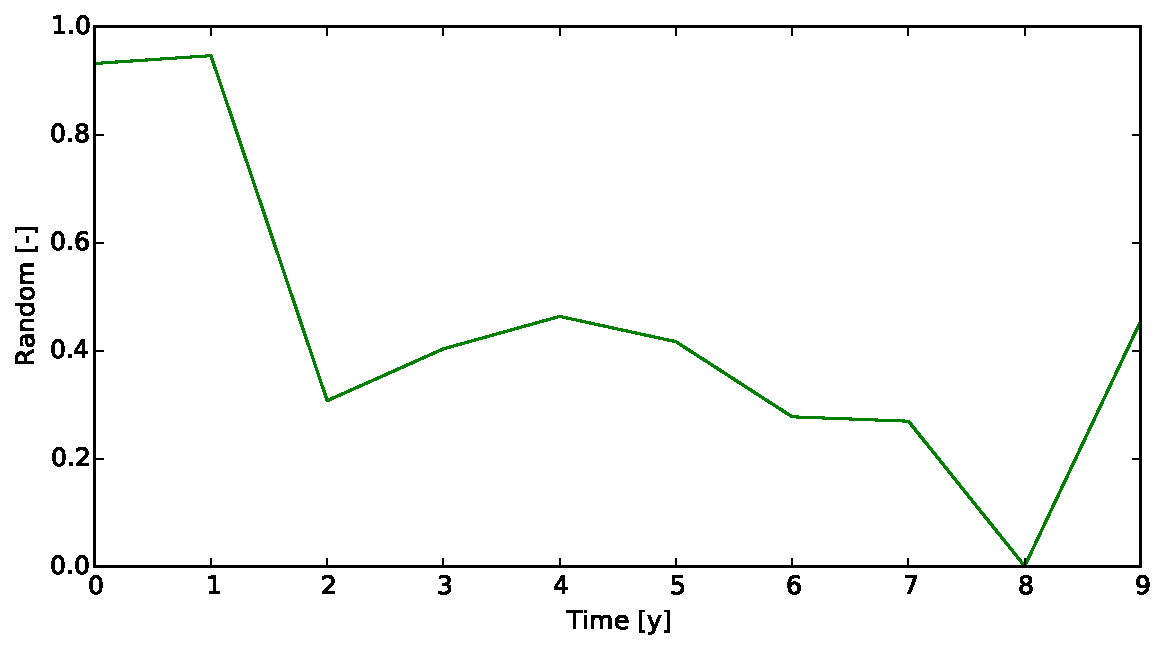
\includegraphics[width=0.48\textwidth]{plot1}
				\caption{Side Cap figure \capunit{\celsius}.
				\label{fig:plot1SC}}
\end{SCfigure}

\lipsum[18]




\singlefig{plot1}{singlefig: Caption}

\doublefig{plot2}{doublefig: Caption 1}{plot3}{doublefig: Caption 2}

\lipsum[18]



\begin{figure}[h!tb]
        \centering
        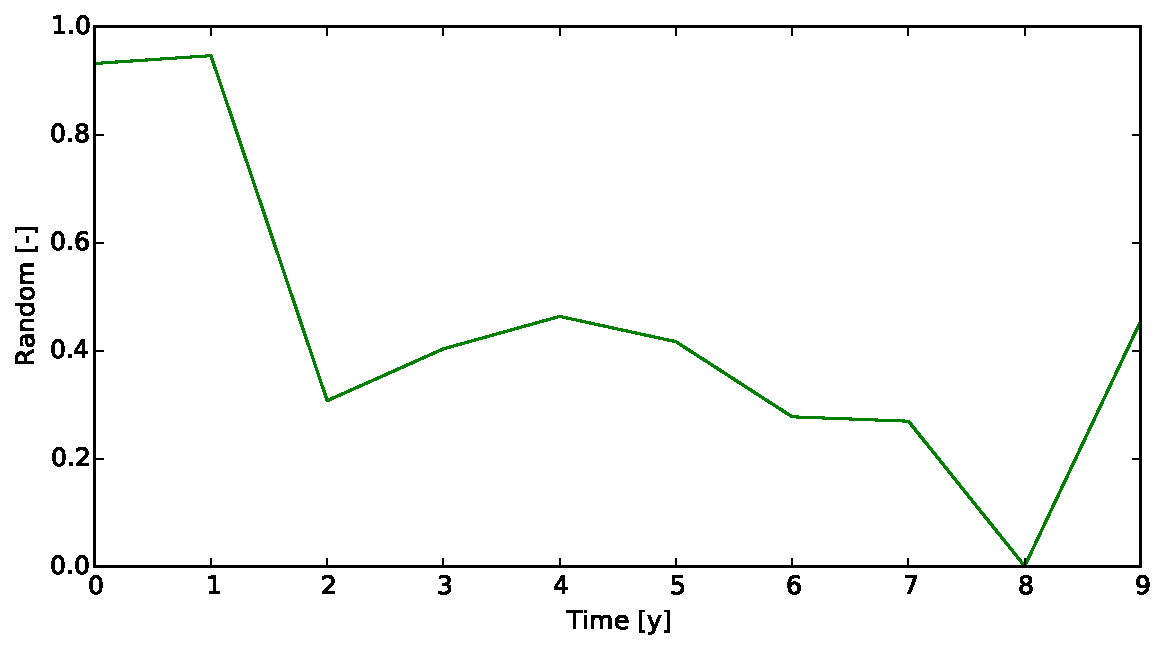
\includegraphics[width=\textwidth]{plot1}   
	\caption{Normal figure. \label{fig:plot1N}}
\end{figure}


\lipsum[19]

\begin{figure}[h!tb]
\begin{tikzpicture}
\begin{axis}[scale only axis, width=0.1pt, height=0.1pt, ymin=0, ymax=3, xmin=0, xmax=5, ticks=none, ytick = \empty, legend style = {font=\sansmath\sffamily\small}, area legend, legend pos=south west, axis lines = none,legend to name = leg,legend columns = -1]

% LEGEND
	\addlegendimage{black,fill= red}
	\addlegendimage{black,fill= white}
	\addlegendimage{black,fill= blue}
	\addplot coordinates{(0,0)};
		\legend{{$\Delta$LH $> 0$\hspace*{2pt}},{$\Delta$LH $\approx 0$\hspace*{2pt}}, $\Delta$LH $< 0$}
	\end{axis}


	\node[inner sep = 0pt] (fig) {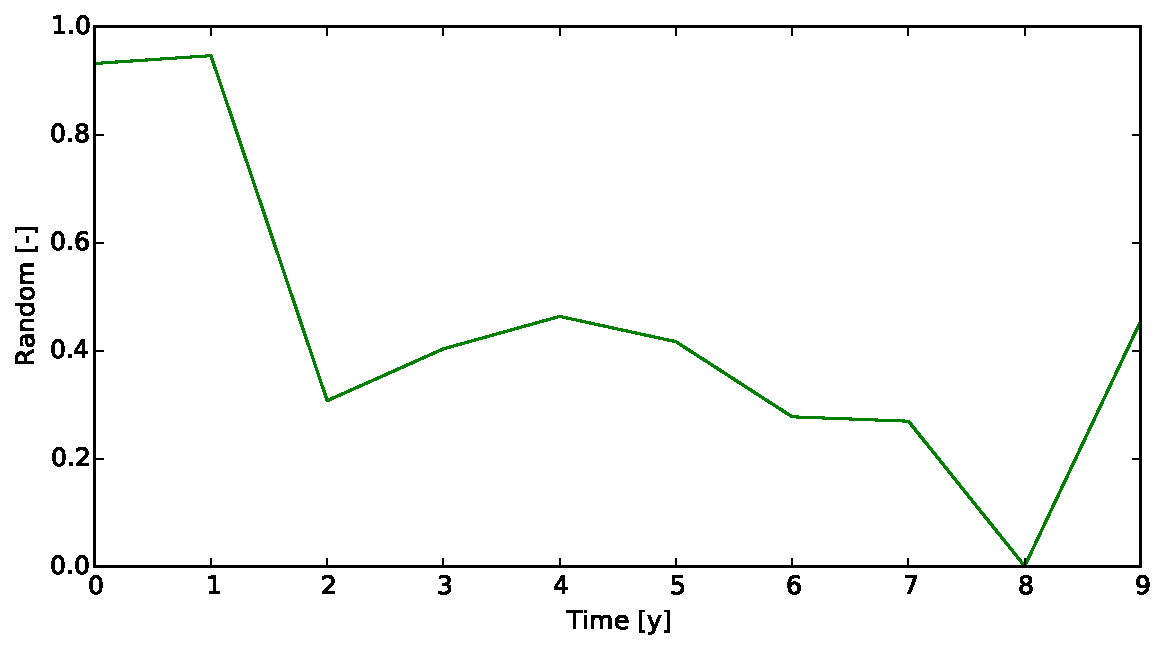
\includegraphics[angle=0,width=\textwidth]{plot1}};

\path[draw,semithick,white] (fig.south west) ++(1.31,2.11) rectangle +(0.3cm,0.3cm);

\node[below] at (fig.south) {\pgfplotslegendfromname{leg}};

% INSET

\node[anchor=south west,xshift=2.5cm,yshift=1.5cm] (ct) at (fig.south west) {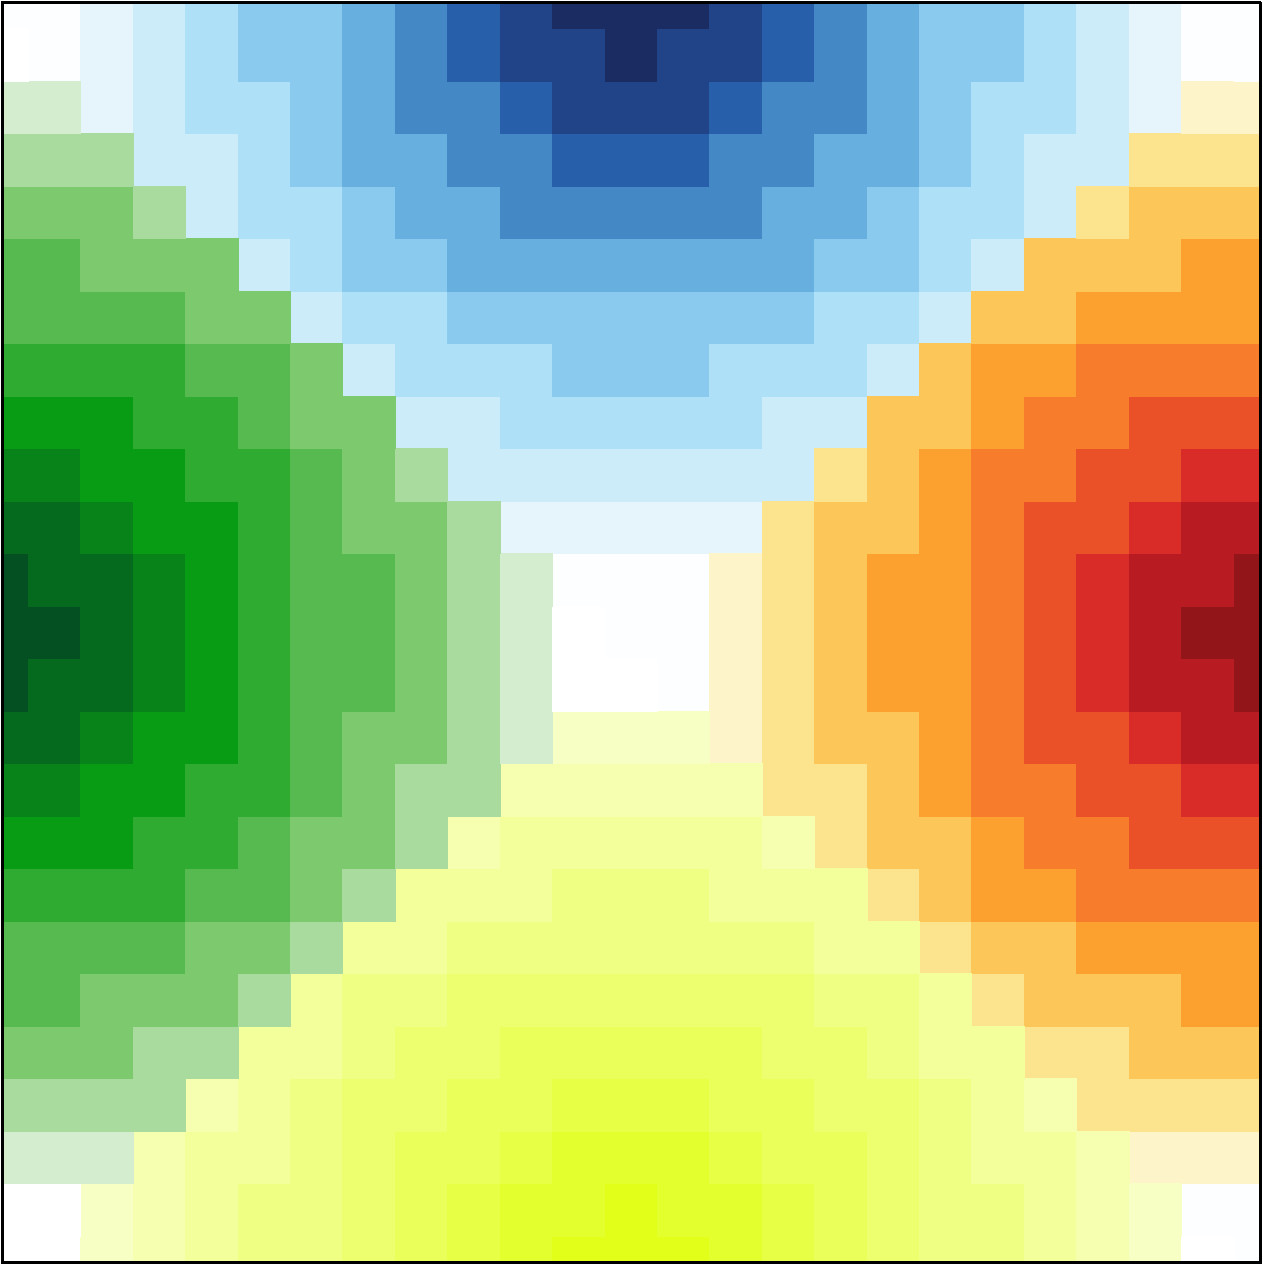
\includegraphics[width=0.1\textwidth]{colortable}};
\begin{scope}[font = \scriptsize\sansmath\sffamily, inner sep = 2pt]
	\begin{scope}[left]
		\node at (ct.north west) {$1$};
		\node (rhoSW) at (ct.west) {$0$};
		\node at (ct.south west) {$-1$};
	\end{scope}
	\node[rotate=90,above] at (rhoSW.west) {$\rho_{LH, SW}$};

	\begin{scope}[above]
		\node at (ct.north west) {$-1$};
		\node (rhoP) at (ct.north) {$0$};
		\node at (ct.north east) {$1$};
	\end{scope}
	\node[above] at (rhoP.north) {$\rho_{\text{LH,P}}$};
\end{scope}
\end{tikzpicture}

\captionof{figure}{Hand-made legend with pgfplots and labeled inset with tikz.}				
 
\end{figure}



\lipsum[20]


\subsection{Water Balance} \label{sec:wBal}

\lipsum[21]

\begin{figure}[h!tb]
\begin{tikzpicture}
\node (CTRL)    {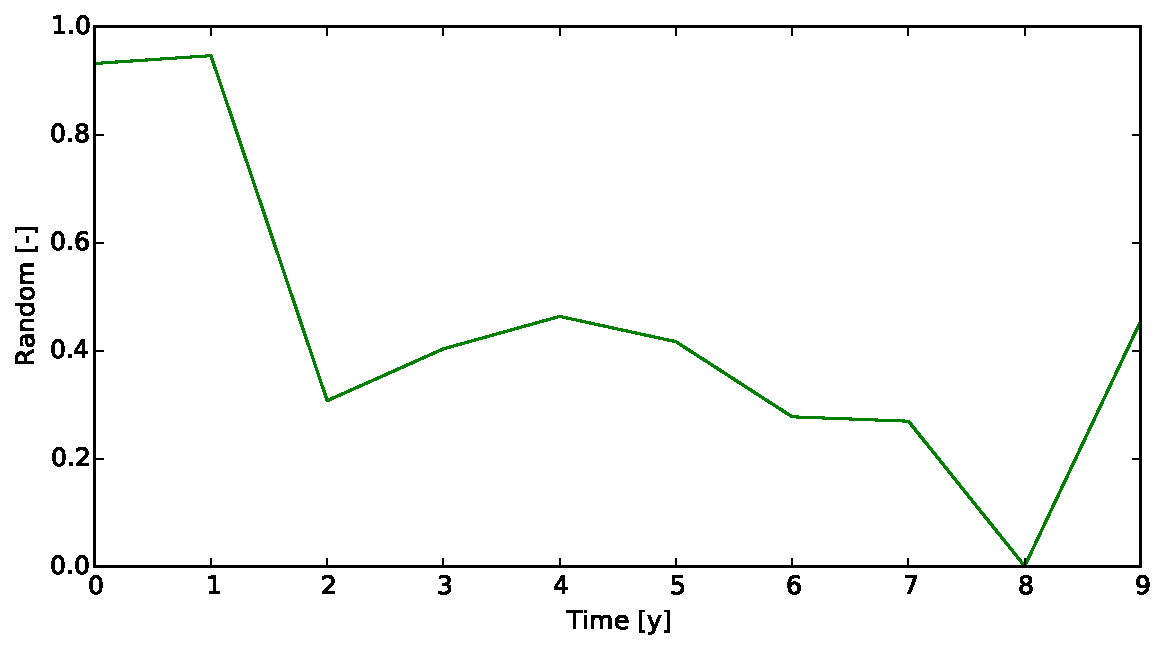
\includegraphics[width=0.310\textwidth]{plot1}};
\node[anchor=south west] (MIN) at (CTRL.south east) {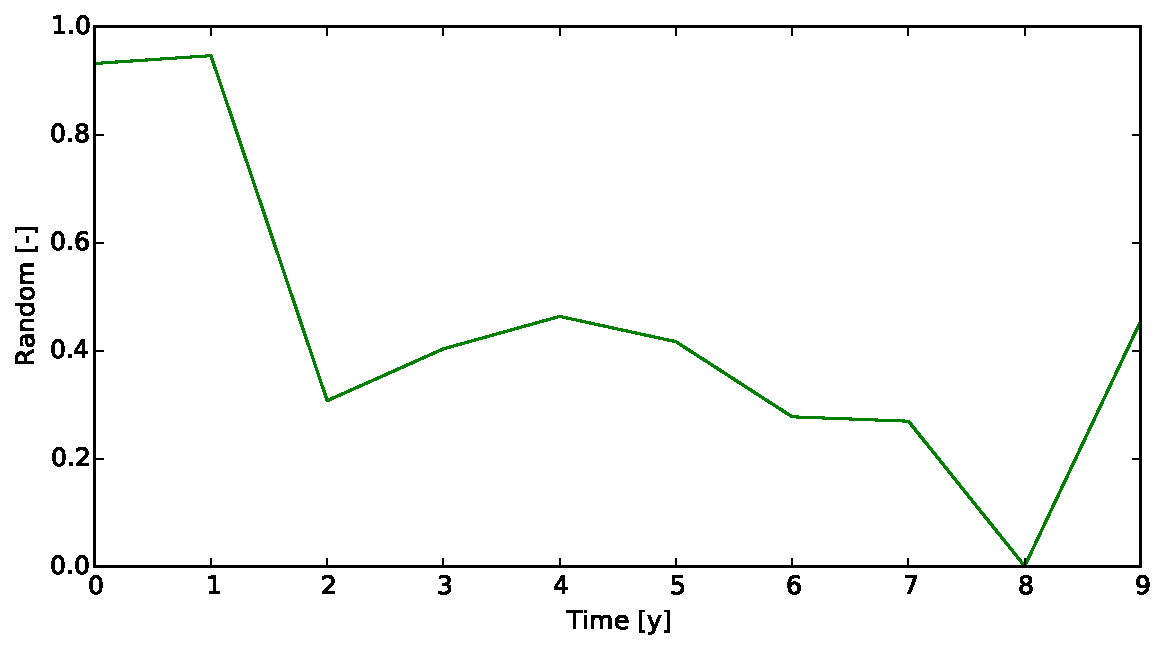
\includegraphics[width=0.310\textwidth]{plot1}};
\node[anchor=south west] (MAX) at (MIN.south east)   {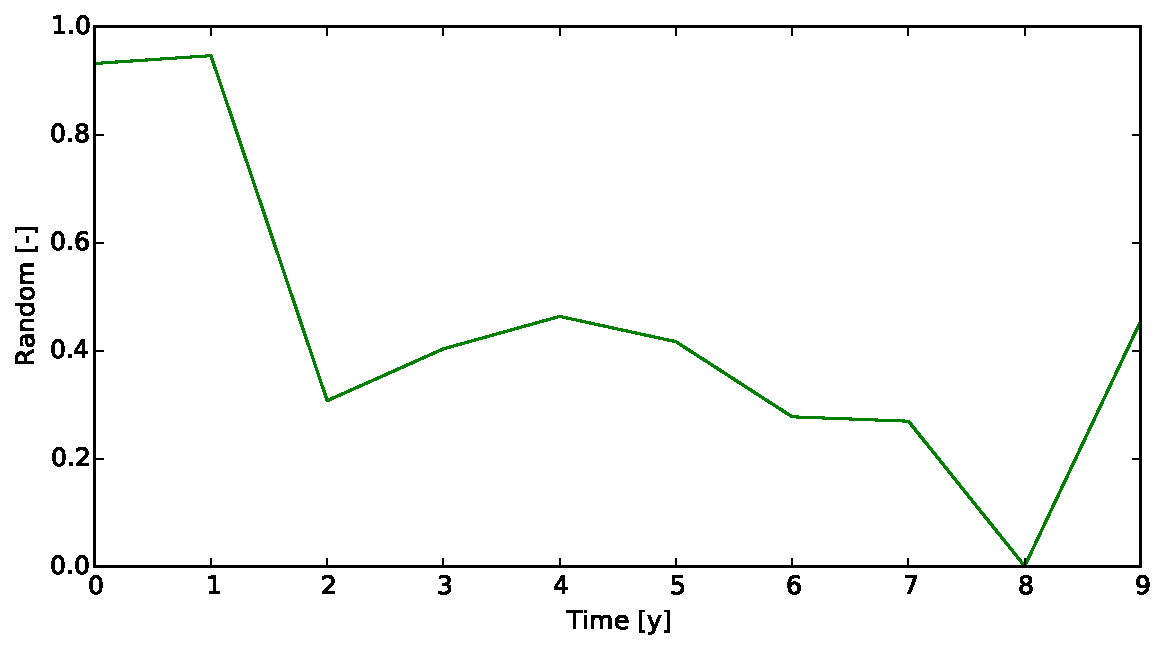
\includegraphics[width=0.310\textwidth]{plot1}};
\node[anchor=north,font=\sansmath\sffamily\small] at (CTRL.north west) {(a)};
\node[anchor=north east,font=\sansmath\sffamily\small] at (MIN.north west) {(b)};
\node[anchor=north west,font=\sansmath\sffamily\small] at (MAX.north west) {(c)};
\end{tikzpicture}
        \caption{Three subfigures produced with tikz.}
\end{figure}

\lipsum[22]

%\cleardoublepage
%\input{ConclusionOutlook}
%%\cleardoublepage
%\vfill
%\input{Various} % -> declaration of originality, acknowledgement
%\cleardoublepage
%\appendix
%\input{Appendix}

%\setcounter{figure}{0}
%\clearpage
%\input{MethodsAppendix}
%\input{AddMaterial}
%\pagestyle{plain}
%% The Bibliography
%\cleardoublepage
%\clearpage
%\phantomsection
%\addcontentsline{toc}{section}{References} %'Bibliography' into toc
%\bibliographystyle{ametsoc} %Style of Bibliography
%\bibliographystyle{atmos} %Style of Bibliography

%\bibliographystyle{apa}
%\scriptsize
%\renewcommand{\refname}{}
%\bibliography{./../Bibliography} %You need a file 'literature.bib' for this.


%% Appendix
%\appendix



\end{document}